\chapter{Formale Grammatiken}
\index{Formale Grammatiken}
% TODO: Chomsky-Hierarchie
%
\index{Formale Grammatiken}
Die Informatik macht sich Gedanken um die systematische Verarbeitung von Information. Anhand verschiedener Modelle haben wir bereits gesehen, wie wir eine Eingabe nehmen, diese nach Vorschriftsregeln verarbeiten und dann eine Antwort auf das gestellte Anfangsproblem liefern. Dabei haben wir eine wichtige Frage wegfallen lassen: Woher weiß der Algorithmus, ob diese Eingabe valid? Woher weiß die Turingmaschine, dass das---was auf dem Band steht---eine korrekte Eingabe ist, die zu keinem undefinierten Verhalten führt?\footnote{Als Beispiel für undefiniertes Verhalten sei hier die Division durch Null gegeben.}

Das Wortproblem stellt folgende Frage:
\begin{quotation}
  Gegeben sei eine Sprache $S$. Ermittle, ob ein Wort $W$ Teil von $S$ ist oder nicht.
\end{quotation}
%
Wir verwenden die neuen Begriffe \emph{Wort} (oder String bzw. Zeichenkette) und \emph{Sprache} (Vorschriften über die mögliche Aneinanderreihung von Wörtern). Eine Sprache beschreibt eine Menge von Wörtern\footnote{Beachte, dass Wort anders als im linguistischen Sinn betrachtet wird. So ist ein Satz wie ,,Der Gärtner ist der Mörder`` \emph{ein} Wort der Sprache.}. Für diese muss eine Zugehörigkeitsbeziehung ermittelt werden können. Wir führen das Konzept der Sprachen und Grammatiken ein.

\section{Eine einfache Sprache}
%
Gegeben sei eine einfache Sprache, die genau nur 1 Zeichenkette akzeptieren soll und zwar jene, die nur aus \gramm{a} besteht. Stimmt das Eingabewort $W$ mit der Zeichenkette \gramm{a} überein, wird die Eingabe akzeptiert andernfalls zurückgewiesen. So wird das Wortproblem entschieden. Da wir die Sprache als Menge repräsentieren können, verwenden wir Mengennotation: $S = \{\texttt{a}\}$ und das Wortproblem für einen String $s$ lautet $s \stackrel{?}{\in} S$.
%
\begin{figure}[ht]
 \begin{center}
  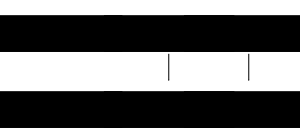
\includegraphics{img/wordproblem.pdf}
  \caption{Zwei Beispiele für die Entscheidung das Wortproblems für die Sprache \gramm{a}.}
  \label{fig:wordproblem}
 \end{center}
\end{figure}

Ein komplexeres Beispiel verwendet mehrere Zeichen: Die Sprache $T$ als \gramm{abb} akzeptiert genau jene Wörter, die eine Länge 3 und den Aufbau ,,abb`` haben.

Wir möchten in diesem Kapitel also Sprachen definieren. Wir haben eine textuelle Beschreibung verwendet. Wir haben auch Mengennotation verwendet. Wobei diese Ansätze durchaus legitim sind, besitzt der textuelle Ansatz das Problem fehleranfällig zu sein (Spezialfälle werden nicht spezifiziert) und Mengennotation kann komplexere, unendliche Sprachen nicht übersichtlich abbilden. Wir befassen uns daher mit zwei weiteren Ansätzen in den folgenden Abschnitten:
\index{Reguläre Ausdrücke}
\begin{itemize}
  \item reguläre Ausdrücke (kompakte Schreibweise für eine bestimmte Untermenge von Sprachen)
  \item formale Grammatiken (ein mächtiges Werkzeug um allgemeine Grammatiken zu beschreiben)
\end{itemize}

\subsubsection*{Unsere einfachen Sprachen in Mengennotation}
\[
  S = \{\texttt{a}\}  \qquad  T = \{\texttt{abb}\}
\]

\subsubsection*{Unsere einfachen Sprachen als regulärer Ausdruck}
\lstset{language={}, label={lst:regex_S}, caption={$S$ als regulärer Ausdruck}, frame={single}}
\begin{lstlisting}
a
\end{lstlisting}
\lstset{language={}, label={lst:regex_T}, caption={$T$ als regulärer Ausdruck}, frame={single}}
\begin{lstlisting}
abb
\end{lstlisting}

\subsubsection*{Unsere einfachen Sprachen als formale Grammatik}
\lstset{language={}, label={lst:regex_S}, caption={$S$ als formale Grammatik $G=(V,\Sigma,P,S)$}, frame={single}, escapechar=\@}
\begin{lstlisting}
S @$\rightarrow$@ a
\end{lstlisting}
\lstset{language={}, label={lst:regex_T}, caption={$T$ als formale Grammatik $G=(V,\Sigma,P,S)$}, frame={single}, escapechar=\@}
\begin{lstlisting}
S @$\rightarrow$@ abb
\end{lstlisting}

\section{Eine Grammatik mit Wiederholungen}
%
Wir möchten unsere Sprachendefinitionen erweitern, indem wir eine Anzahl abbilden können. So war es uns bislang nicht möglich eine Sprache (zB) ,,Akzeptiere alle Wörter die nur aus \emph{a}s bestehen`` zu formulieren. Hierfür müssen wir Wiederholungen repräsentieren.

\subsection{In regulären Ausdrücken}
%
Wir führen daher das Konzept der Quantoren ein. Ein regulärer Ausdruck ist eine Zeichenkette, die ein oder mehrere Zeichenketten spezifiziert. Grundsätzlich wird für reguläre Ausdrücke jenes Wort notiert, welches innerhalb der Sprache liegt. Wir lernen jetzt Konzepte kennen, um mehrere Wörter abzubilden.
%
\begin{table}[ht]
 \begin{center}
  \begin{tabular}{cl}
   \hline
    \texttt{+} & Das vorige Zeichen kommt 1--$\infty$ mal vor (,,1-mal oder öfters``) \\
    \texttt{*} & Das vorige Zeichen kommt 0--$\infty$ mal vor (,,beliebig oft``) \\
    \texttt{?} & Das vorige Zeichen kommt 0--1 mal vor (,,optional``) \\
   \hline
  \end{tabular}
  \caption{Quantoren in regulären Ausdrücken}
  \label{tab:quantifiers}
 \end{center}
\end{table}

\index{Quantoren (reguläre Ausdrücke)}
In Tabelle~\ref{tab:quantifiers} werden Quantoren definiert. Kommen diese Zeichen in einem regulären Ausdruck vor, werden diese nicht wortwörtlich verstanden, sondern beziehen sich auf das letzte Zeichen oder die letzte Gruppe.

Wir betrachten ein Beispiel. Gesucht sei folgende Grammatik $R$:
\begin{quote}
  Das Zeichen \gramm{a} kann (aber muss nicht) vorkommen. Nachfolgend kommt ein \gramm{b} und
  anschließend beliebig viele \gramm{c}.
\end{quote}

Der folgende Ausdruck spezifiziert diese Grammatik:
\lstset{language={}, label={lst:regex_repetition}, caption={Die Grammatik $\{a^n b c^m | 0\leq n\leq 1, m \geq 0\}$}, frame={single}}
\begin{lstlisting}
a?bc*
\end{lstlisting}

Das erste Fragezeichen bezieht sich auf das vorige Zeichen ,,a`` und macht es optional. Das folgende ,,b`` muss zwingend vorkommen. Dem ,,c`` ist ein Stern nachgestellt und ein Stern spezifiziert die Quantität ,,beliebig oft``.

\subsection{In Mengennotation}
%
Die Beschriftung von Listing~\ref{lst:regex_repetition} nutzt Mengennotation. Hierbei wird die Anzahl der Vorkommnisse eines Zeichens oder einer Gruppe mit einer hochgestellten Zahl notiert. Wird die Domäne der Variable ($n$ und $m$) nicht angegeben, spricht man von natürlichen Zahlen inklusive der 0.

\subsection{Als formale Grammatik}
%
In einer formalen Grammatik ist Wiederholung über Rekursion abzubilden.

Aber besprechen wir zuerst, was formale Grammatiken denn sind und wie sie Wörter erzeugen. Eine formale Grammatik $G = (V, \Sigma, P, S)$ besitzt ein endliches Vokabular $V$, ein Alphabet $\Sigma$, Produktionsregeln $P$ und ein Startsymbol $S$. Das Erzeugen von Strings startet stets mit dem Startsymbol $S$ und Produktionsregeln $P$ erlauben es uns Zeichen sukzessive durch Zeichen aus $V$ zu ersetzen. Wir unterscheiden dabei zwischen den Terminalsymbolen $\Sigma$ und Nonterminalsymbolen $V \setminus \Sigma$. Terminalsymbole sind jene Symbole, die in der endgültigen Zeichenkette vorkommen. Für Nonterminalsymbole sind Regeln in $P$ definiert, wie man sie ersetzen kann. Die Ersetzungen erfolgen so lange bis nur mehr Terminalsymbole enthalten sind.

% TODO: ,` and ,,`` in wrong order
Als ersten Schritt (um $R$ zu definieren) beschreiben wir eine Grammatik ,Das Zeichen \gramm{a} kann vorkommen`.
\lstset{language={}, label={lst:regex_R1}, caption={$R1$ als formale Grammatik $G=(V,\Sigma,P,S)$}, frame={single}, escapechar=\@}
\begin{lstlisting}
S @$\rightarrow$@ a
S @$\rightarrow$@
\end{lstlisting}

Wir starten also mit einem Startsymbol ,,S`` und ersetzen es jetzt. Entweder wir entscheiden uns für die Zeile 1 und setzen ,,a`` ein oder einen leeren String ,,`` (Zeile 2).

Als zweiten Schritt beschreiben wir eine Grammatik ,Das Zeichen \gramm{a} kann vorkommen. Nachfolgend kommt ein \gramm{b}`.
\lstset{language={}, label={lst:regex_R2}, caption={$R2$ als formale Grammatik $G=(V,\Sigma,P,S)$}, frame={single}, escapechar=\@}
\begin{lstlisting}
S @$\rightarrow$@ ab
S @$\rightarrow$@ b
\end{lstlisting}

Nachdem ein optionales \texttt{a} angegeben wurde, folgt ein \texttt{b}. Für die Wiederholung von \texttt{c} verwenden wir ein Nonterminalsymbol \texttt{R} (welches per Konvention großgeschrieben wird).
\lstset{language={}, label={lst:regex_R3}, caption={$R$ als formale Grammatik $G=(V,\Sigma,P,S)$}, frame={single}, escapechar=\@}
\begin{lstlisting}
S @$\rightarrow$@ abR
S @$\rightarrow$@ bR
R @$\rightarrow$@
R @$\rightarrow$@ cR
\end{lstlisting}

Gehen wir die Produktionsregeln für den Eingabestring \texttt{abcc} durch. Wir starten wieder mit dem Startsymbol ,,S``. Wir ersetzen es mittels der 1. Zeile zu ,,abR``. Wir erkennen ein verbleibendes Nonterminal in ,,R`` in dem String und suchen uns hierfür entsprechende Regeln; die Regeln 3 und 4 kommen in Frage. Für den gegebenen Eingabestring müssen wir Regel 4 verwenden. Es entsteht der String ,,abcR``. Wieder ersetzen wir das ,,R`` durch die Regel 4. ,,abcR`` besitzt auch noch ein Nonterminal, welches jetzt jedoch mittels Regel 3 ersetzt wird. Es entsteht der String ,,abcc`` (bestehend nur aus Terminalsymbolen). Damit liegt der String ,,abcc`` in der durch die formale Grammatik spezifizierten Sprache.

\section{Alternation in Grammatiken}
%
Gesucht sei folgende Grammatik $A$:
\begin{quote}
  Die Zeichenkette beginnt mit ,,message of the `` und endet entweder mit ,,day`` oder ,,week``. Am Ende befindet sich weiters ein Rufzeichen ,,{!}``.
\end{quote}

\subsection{Als regulärer Ausdruck}
%
In einem regulären Ausdruck lässt sich eine Alternation definieren, indem der vertikale Balken als Alternationsoperator verwendet wird. Dabei wird entweder die linke Seite vom Balken oder die rechte Seite herangezogen. Die Seiten können durch eine Gruppierung beschränkt werden, die durch runde Klammern definiert wird.

\lstset{language={}, label={lst:regex_alternation}, caption={Die Grammatik $A$}, frame={single}}
\begin{lstlisting}
message of the (day|week)!
\end{lstlisting}

\subsection{Als formale Grammatik}
%
Alternation haben wir schon implizit bei formalen Grammatiken kennen gelernt. Wir wählen aus mit welcher Regel wir ein Nonterminalsymbol ersetzen.
%
\lstset{language={}, label={lst:regex_A}, caption={$A$ als formale Grammatik $G=(V,\Sigma,P,S)$}, frame={single}, escapechar=\@}
\begin{lstlisting}
S @$\rightarrow$@ message of the A!
A @$\rightarrow$@ day
A @$\rightarrow$@ week
\end{lstlisting}

Wir haben jetzt die wichtigsten Konzepte betrachtet, um Sprachen definieren zu können. Wir möchten jetzt noch auf ein paar spezifische Details eingehen und die Mächtigkeit von Sprachen evaluieren.

\section{Reguläre Ausdrücke}
%
\begin{table}[ht]
 \begin{center}
  \begin{tabular}{cl}
   \hline
    \texttt{.}     & Ein beliebiges Zeichen (aus $\Sigma$) \\
    \texttt{[ab]}  & Eines der Zeichen aus $\set{\texttt{a}, \texttt{b}}$ (Zeichenmenge) \\
    \texttt{(ab)}  & Fasst die Sequenz ,,ab`` zu einer Gruppe zusammen (Gruppierung) \\
    \texttt{a|bc}  & Entweder ,,a`` oder ,,bc`` (Alternation) \\
    \texttt{+}     & Das vorige Zeichen kommt 1--$\infty$ mal vor (,,1-mal oder öfters``) \\
    \texttt{*}     & Das vorige Zeichen kommt 0--$\infty$ mal vor (,,beliebig oft``) \\
    \texttt{?}     & Das vorige Zeichen kommt 0--1 mal vor (,,optional``) \\
   \hline
  \end{tabular}
  \caption{RegEx Operatoren}
  \label{tab:regex_op}
 \end{center}
\end{table}
%
Reguläre Ausdrücke (engl. ,,regular expressions`` oder kurz RegEx) sind eine kompakte Schreibweise, um mehrere Zeichenketten darzustellen. In Tabelle~\ref{tab:regex_op} sind die Sonderzeichen nochmals zusammengefasst dargestellt. In der Tabelle wird eine Möglichkeit genannt eine Zeichenmenge anzugeben. Dieses Konzept kann genauso durch eine Alternation simuliert werden.

\subsection{Non-greedy Verhalten}
%
Maschinen, die reguläre Ausdrücke verarbeiten arbeiten unterschiedlich bzw. können über Modifiers konfiguriert werden. Alte Implementierungen nutzen Backtracking-Verfahren und neuere Implementierungen enthalten Optimierungen, die neu erforscht wurden. Die wesentliche Frage ist, wie diese Maschinen implementiert sind, da sie das Verhalten der regulären Ausdrücke bestimmen.

Eine häufig vorkommende Struktur bei regulären Ausdrücken ist \texttt{(.*)}. Es handelt es sich um eine Gruppe von beliebigen Zeichen beliebiger Länge. Salopp gesprochen matcht dieser Ausdruck jeden String.
Wie sieht es nun mit dem regulären Ausdruck \texttt{(.*)(.*)} und der Eingabe ,,abc`` aus? Greedy-Verhalten bezeichnet das Bestreben eines Ausdrucks, möglichst viel Inhalt zu matchen. Entsprechend würde die erste Punkt-Stern-Kombination die gesamte Eingabe matchen, da sie versucht sich alles zuzuweisen. Dies verwirrt viele RegEx-Benutzer, da ein RegEx \texttt{a(.*)a} bei dem Eingabestring ,,abaaba`` nicht ,,aba`` zweimal matcht, sondern einmal ,,abaaba``.

Non-greedy Verhalten kann man meist durch das Anfügen eines Fragezeichens nach dem Gruppenquantor erreichen. Für unser Beispiel wäre etwa \texttt{a(.*?)a} sinnvoll um den String in zwei Teilen zu matchen.

\section{Kontextfreie Grammatiken}
%
Kontextfreie Sprachen sind mächtiger als reguläre Sprachen. Diese Behauptung besagt, dass die Menge der Sprachen die durch reguläre Ausdrücke repräsentiert werden können kleiner als die Menge der Sprachen ist, die mit formalen, kontextfreien Grammatiken spezifiziert werden können. Wir betrachten ein Beispiel.

Gesucht sei folgende Sprache $E$:
\begin{quote}
  Die Anzahl von ,,a`` ist gleich der Anzahl von ,,b``. 
\end{quote}

Probieren wir einen regulären Ausdruck zu finden.
\lstset{language={}, label={lst:cfg_regex1}, caption={Regulärer Ausdruck für die Sprache $E$}, frame={single}}
\begin{lstlisting}
(ab)*
\end{lstlisting}

Die äquivalente formale Grammatik sieht folgendermaßen aus:
\lstset{language={}, label={lst:regex_A}, caption={Sprache $E$ als formale Grammatik}, frame={single}, escapechar=\@}
\begin{lstlisting}
S @$\rightarrow$@ abS
S @$\rightarrow$@
\end{lstlisting}

Bisher war jedoch die Reihenfolge der Zeichen undefiniert. Wir erweitern nun $E$ zur Sprache $F$:
\begin{quote}
  Eine Sequenz von ,,a`` wird von einer Sequenz der gleichen Länge von ,,b`` gefolgt.
\end{quote}
In Mengennotation wäre dies mit $\set{a^n b^n \mid n \in \mathbb{N}, n \geq 0}$ anzugeben.

Durch die Vorgabe der Position bekommen wir ein neues Problem. Wir versuchen es mit folgendem regulären Ausdruck:
\lstset{language={}, label={lst:rep}, caption={Regulärer Ausdruck Versuch für die Sprache $F$}, frame={single}}
\begin{lstlisting}
a*b*
\end{lstlisting}

Das geübte Auge erkennt, dass die Anzahl der erzeugten ,,a`` ungleich der Anzahl von ,,b`` sein kann. Daher repräsentiert dieser reguläre Ausdruck nicht die spezifizierte Sprache. So ist etwa ,,aaab`` in der Sprache des regulären Ausdrucks enthalten, aber nicht in der textuellen Beschreibung. Wir erkennen, dass die vorliegende Grammatik sich nicht mehr regulär abbilden lässt, sondern ,,kontextfrei`` ist.

Mithilfe einer formalen Grammatik können wir diese Sprache definieren:
\lstset{language={}, label={lst:lang_F}, caption={Formale Grammatik für Sprache $F$}, frame={single}, escapechar=\@}
\begin{lstlisting}
S @$\rightarrow$@ aSB
S @$\rightarrow$@
\end{lstlisting}




\lstset{language={}, label={lst:cfgsample}, caption={Die kontext-freie Grammatik $\set{a^n b^n}$}, escapechar={}, frame={single}}
\begin{lstlisting}
S ::= aSb | $
\end{lstlisting}

Basierend auf S können wir jetzt beliebige Wörter der Sprache ableiten
\lstset{language={}, label={lst:cfl}, caption={Die Ableitung von ,,aaabbb``}, frame={single}}
\begin{lstlisting}
S
aSb
aaSbb
aaaSbbb
aaa$bbb
aaabbb
\end{lstlisting}

Für kontextfreie Grammatiken dürfen wir Nonterminale definieren, die ersetzt werden. Wir müssen dabei beachten, dass wir auf der linken Seite nur ein Nonterminal verwenden dürfen. % TODO: What are the exact rules?

\section{Kontext-sensitive Grammatik}
%
Eine weitere Ebene stellen die kontext-sensitiven Grammatiken dar. Dazu sei folgende Grammatik zu formulieren:
\[
  \set{a^n b^n c^n \mid n \in \mathbb{N}, n \geq 0}
\]

Unser erster Versuch schlägt fehl: Die Anzahl der ,,a`` und ,,b`` sind äquivalent, aber die ,,c`` sind unabhängig. Folglich kann die formulierte Sprache nicht ihre spezifizierte Grammatik einhalten.
\lstset{language={}, label={lst:cflcsl}, caption={Die kontext-freie Grammatik für ein kontext-sensitives Problem}, frame={single}}
\begin{lstlisting}
S ::= aSbB | $
B ::= Bc
\end{lstlisting}

Wir müssen unsere Grammatik ausbauen und auf der linken Seite sowohl Terminale als auch Non-Terminale verwenden:
\lstset{language={}, label={lst:cslsample}, caption={Die kontext-freie Grammatik $\set{a^n b^n c^n}$}, frame={single}}
\begin{lstlisting}
S ::= aSBH | $
aS ::= aa
aB ::= ab
bB ::= bb
HB ::= BC
bC ::= bc
cC ::= cc
CH ::= CC
\end{lstlisting}

\section{Chomsky-Hierarchie}
%
Wir haben bei diesen Beispielen gesehen, dass gewisse Modelle nicht ausreichen, um Sprachen zu beschreiben. Noam Chomsky hat die Chomsky-Hierarchie formuliert, um Sprachen in Kategorien einzuteilen. Dabei sind reguläre Sprachen die schwächsten Sprachen. Kontextfreie Sprachen stehen über den regulären Sprachen und können auch alle regulären Sprachen abbilden. Am mächtigsten sind die rekursive-aufzählbaren Sprachen, die es etwa erlauben die Anzahl der Rekursionen in den Ersetzungsregeln während der Verarbeitung zu verändern.

Abbildung~\ref{fig:chomsky_hierarchy} visualisiert die Chomsky-Hierarchie.
%
\begin{figure}[ht]
 \begin{center}
  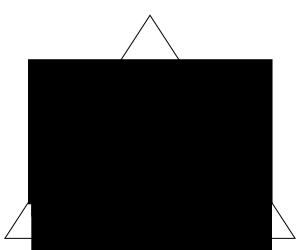
\includegraphics{img/chomsky_hierarchy.pdf}
  \caption{Die Chomsky-Hierarchie}
  \label{fig:chomsky_hierarchy}
 \end{center}
\end{figure}
